\documentclass[a4paper, 12pt]{article}%тип документа

%Русский язык
\usepackage[T2A]{fontenc} %кодировка
\usepackage[utf8]{inputenc} %кодировка исходного кода
\usepackage[english,russian]{babel} %локализация и переносы

%отступы 
\usepackage[left=2cm,right=2cm,top=2cm,bottom=3cm,bindingoffset=0cm]{geometry}

%Вставка картинок
\usepackage{graphicx}
\graphicspath{}
\DeclareGraphicsExtensions{.pdf,.png,.jpg, .jpeg}

%Таблицы
\usepackage[table,xcdraw]{xcolor}
\usepackage{booktabs}

%Графики
\usepackage{pgfplots}
\pgfplotsset{compat=1.9}

%Математика
\usepackage{amsmath, amsfonts, amssymb, amsthm, mathtools}

%Заголовок
\author{Подлесный Артём \\ группа 827}
\title{ЗАДАЧА ТРЁХ ТЕЛ \\ Формулировка, современное состояние}

\begin{document}
\maketitle

\paragraph{Задача трёх тел}  (в астрономии) --- одна из задач небесной механики, состоящая в определении траекторий движения трёх тел (материальных точек), взаимодействующих по закону тяготения Ньютона. В отличие от задачи двух тел, в общем случае задача не имеет решения в виде конечных аналитических выражений.
\section{Формулировка}
Общая задача трёх тел в небесной механике описывается системой обыкновенных дифференциальных уравнений второго порядка:
\begin{equation}
\begin{cases}
\ddot{\vec{q_1}}=\gamma m_2\dfrac{\vec{q_2}-\vec{q_1}}{|\vec{q_2}-\vec{q_1}|^3}+\gamma m_3\dfrac{\vec{q_3}-\vec{q_1}}{|\vec{q_3}-\vec{q_1}|^3}\\
\ddot{\vec{q_2}}=\gamma m_1\dfrac{\vec{q_1}-\vec{q_2}}{|\vec{q_1}-\vec{q_2}|^3}+\gamma m_3\dfrac{\vec{q_3}-\vec{q_2}}{|\vec{q_3}-\vec{q_2}|^3}\\
\ddot{\vec{q_3}}=\gamma m_1\dfrac{\vec{q_1}-\vec{q_3}}{|\vec{q_1}-\vec{q_3}|^3}+\gamma m_2\dfrac{\vec{q_2}-\vec{q_3}}{|\vec{q_2}-\vec{q_3}|^3},
\end{cases}
\end{equation}

где $\gamma$  --- гравитационная постоянная, $m_i$ --- массы тел, $\vec{q_i}$ --- радиус-векторы, определяющие их положение.
\subsection{Возможность общего решения}
Брунс и Пуанкаре доказали, что в общем случае систему дифференциальных уравнений для движения трёх тел невозможно свести к интегрируемой, разложив её на независимые уравнения. Система уравнений для трех тел соответствует фазовому потоку в 18-мерном фазовом пространстве, а теоремы Генриха Брунса и Анри Пуанкаре показывают, что траектории в фазовом пространстве ведут себя крайне запутанно. Исходя из этого, пока не удалось получить аналитического решения задачи трёх тел. Мои рассуждения на тему получения решения такой математической задачи достаточно бессмысленны, так как я не обладаю достаточными знаниями в этой области, поэтому в своём докладе я сосредоточился на демонстрации частных решений этой задачи и подходе к ней в современной науке.
\subsection{Приближенные решения}
Проблему нахождения решения задачи трёх тел стоит рассматривать именно как математическую проблему. Идея алгоритма нахождения приближенного решения была предложена Вейерштрассом в 1885 году в виде задачи:

Пусть дана система произвольного числа материальных точек, взаимодействующих по закону Ньютона. Требуется, в предположении, что не произойдет соударения каких-либо двух точек, представить координаты каждой точки в виде рядов по каким-либо непрерывным функциям времени, равномерно сходящихся для всех действительных значений этой переменной.

Иными словами требуется получить выражение для координат тел в виде
\[\lim\limits_{n\to \infty} P_n(t) ,\]
где $P_n(t)$ -- некоторые полиномы. Существование таких полиномов сразу следует из непрерывности решения, но найти конструктивный способ отыскания полиномов до сих пор не удалось. Обсуждение самой возможности ситуации, описанной в задаче Вейерштрасса, привело к ряду важных теорем:
\paragraph{Теорема Пенлеве:} если решение задачи трёх тел является аналитической функцией $t$ в интервале $[0,t_{0})$, но перестает быть таковым при $t=t_{0}\neq\infty$, то при $t\to t_0 -0$ или все расстояния между телами стремятся к нулю (тройное соударение тел), или одно из них стремится к нулю, а остальные два — к конечным пределам (простое соударение тел).
\paragraph{Теорема Слудского:} тройное соударение в задаче трёх тел возможно лишь при условии обращения в нуль момента импульса системы и, следовательно, может иметь место лишь при весьма специальных начальных данных.

Эти ограничения привели к представлению решения залачи трёх тел в виде сходящихся рядов в работе Карла Сундмана. Он нашёл алгоритм нахождения коэффициентов для таких рядов.
\paragraph{Теорема Сундмана:} Если момент импульса системы не равен нулю, то существует так называемый регуляризирующий параметр $s$, через который можно выразить координаты и время аналитическим образом в окрестности вещественной оси $s$.

Однако несмотря на найденный алгоритм, для того, чтобы применять такое решение в практической вычислительной астрономии, нужно брать слишком большое число членов ряда. По крайней мере в случае Лагранжа для нужд вычислительной астрономии в сходящихся рядах Зундмана нужно брать как минимум $10^{8\cdot10^6}$ членов, что значительно осложняет применение этого метода на практике. Именно поэтому, на данный момент открыто достаточно мало частных решений этой задачи, которые опираются на другие методы. 
\section{Частные решения}
\subsection{Традиционные решения}
В течение трехсот лет, до 2013 года, было известно только три вида периодических орбит: семейство траекторий Эйлера-Лагранжа, семейство Бруке-Хено-Хаджидеметриу и восьмерка Мура. Рассмотрим их подробнее.
\paragraph{Семейство Эйлера-Лагранжа}
В 1772 г. Лагранж опубликовал свой знаменитый мемуар «О задаче трех тел», удостоенный впоследствии премии Парижской академии наук. В нем, занимаясь уравнениями задачи
трех тел, Лагранж, между прочим, указывает на существование двух классов движений в задаче трех тел, которые описываются несложными математическими формулами.
Для движений одного класса три взаимно притягивающиеся по закону Ньютона точки
$P_1$, $P_2$ и $P_3$, расположенные в вершинах равностороннего треугольника произвольных размеров, при определенных по величине и на правлению скоростях будут и в последующем двигаться, постоянно образуя равносторонний треугольник. Изменение его стороны со временем
и вращение вокруг центра масс можно определить, пользуясь законами Кеплера. Частные решения этого класса называют треугольными, или лагранжевыми, решениями.
В движениях второго класса все три тела постоянно находятся на одной прямой, вращающейся вокруг общего центра масс тел в соответствии со вторым законом Кеплера, а расстояния между телами изменяются опять же по законам кеплеровских движений. Существование таких частных решений было отмечено Эйлером в 1767 г., за пять лет до мемуара Лагранжа. Решения второго класса получили название прямолинейных (коллинеарных), или эйлеровых.
Траектории тел $P_1$, $P_2$ и $P_3$, соответствующие обоим классам решений, по казаны на рисунке 1. Представлен случай эллиптического движения. Точками отмечены положения тел
для трех (и двух) моментов времени соответственно. 
\begin{figure}[h!]
\center{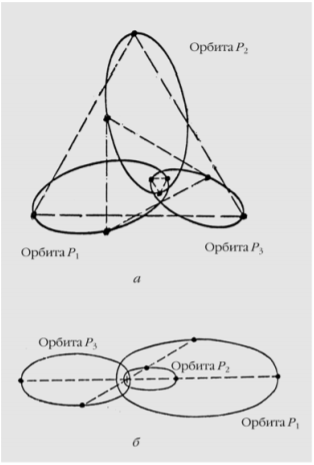
\includegraphics[scale=1.3]{f1.png}}
\caption{Траектории для точных решений задачи трех тел: а -- треугольные решения Лагранжа; б -- прямолинейные решения Эйлера. }
\end{figure}
\paragraph{Семейство Бруке-Хено-Хаджидеметриу и восмерка Мура}
Два следующих решения описывают плоское движение трёх тел, имеющих равные массы, при специфических начальных условиях. Эти траектории представлены на рис 2 и 3.
\begin{figure}[h!]
\center{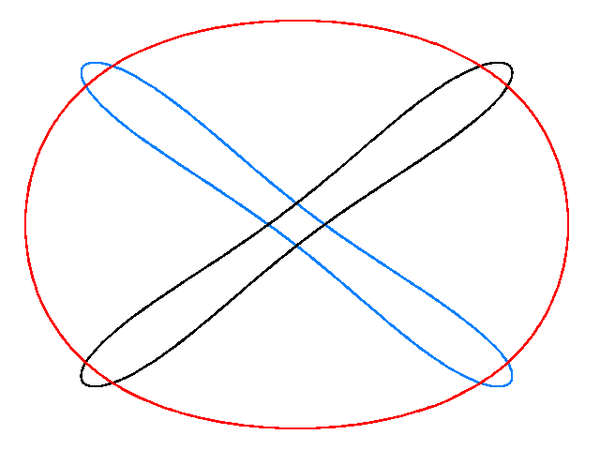
\includegraphics[scale=0.5]{f2.png}}
\caption{Пример орбиты из семейства Бруке-Хено-Хаджидеметриу.}
\end{figure}

\begin{figure}[h!]
\center{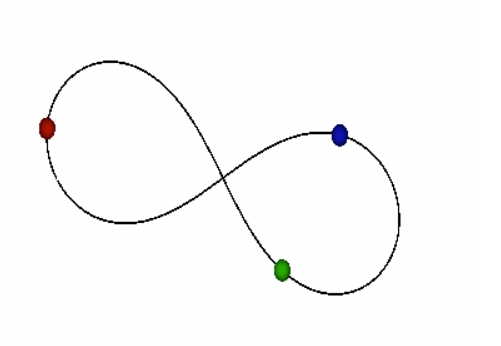
\includegraphics[scale=1.1]{f3.png}}
\caption{Пример орбиты -- восьмерки Мура.}
\end{figure}
\subsection{Современный подход}
Отличие этих традиционных решений от современных в том, что они были получены в виде точного решения строгими математическими методами, и для каждой траектории существует доказательство её существования. В отличие от этого, решения, полученные с 2013 года -- получены с помощью компьютерного моделирования. В 2013 году двое сербских математиков (Милован Шуваков и Велько Дмитрашинович) с помощью численного моделирования обнаружили одиннадцать новых семейств замкнутых траекторий в плоской задаче трех тел с одинаковыми массами и моментами импульса. В 2015 другой сербский математик (Ana Hudomal) сообщила об открытии еще четырнадцати типов орбит. 

И вот, 13 сентября 2017 года китайскими математиками (Xiaoming Li, Yipeng Jing, Shijun Liao) был выпущен препринт статьи, в котором были открыты 1349 новых орбит, включая все предыдущие. В этой же работе они исследовали на устойчивость все предыдущие открытые орбиты. Новые периодические траектории китайские математики искали с помощью разработанного ими метода «чистого численного моделирования» (Clean Numerical Simulation). Для этого они рассматривали начальные конфигурации трех тел одинаковой массы, образующих равнобедренный треугольник, и задавали им различные начальные скорости.

Чтобы найти периодические орбиты, ученые немного шевелили начальные положения тел и смотрели, насколько точно они возвращаются в исходное положение спустя период. Математики считали, что траектория периодична, если величина соответствующей функции отклонения составляла менее $10^{-6}$. Начальные положения, отвечающие интересным траекториям, определялись с помощью метода Ньютона, а потом соответствующие орбиты были аппроксимированы многочленами Тейлора с точностью до $10^{-70}$, что гарантировало их периодичность. Некоторые из этих орбит показаны на рис 4.

\begin{figure}[h!]
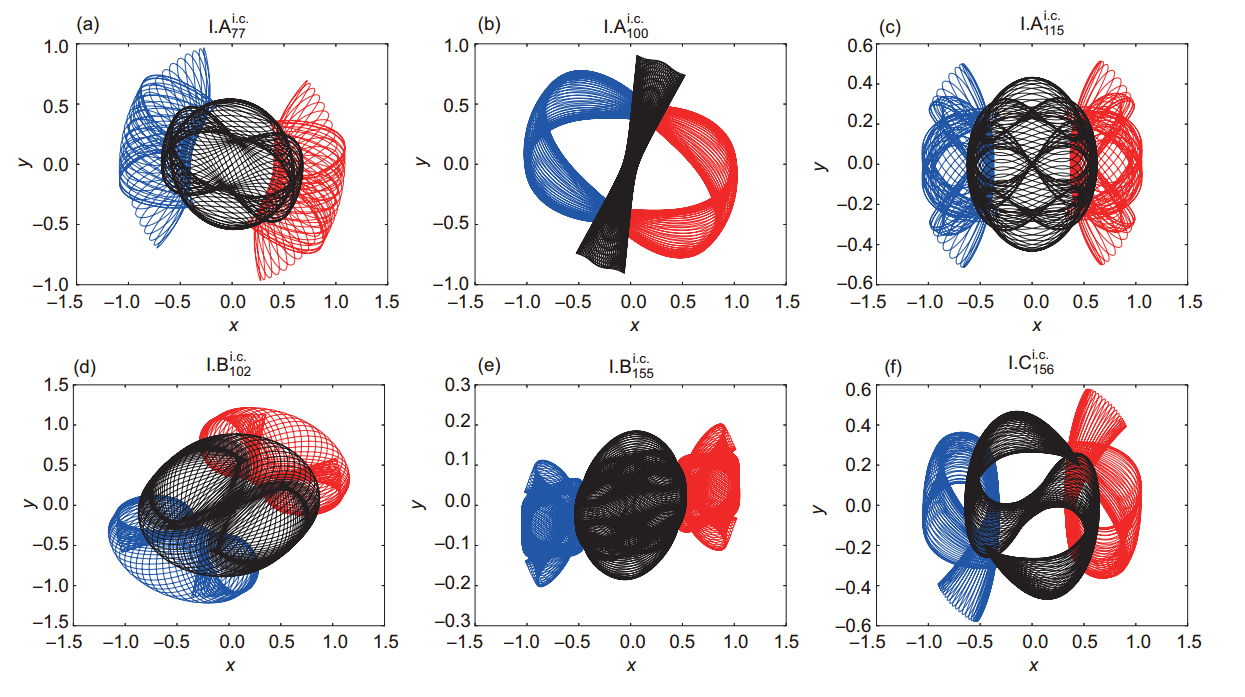
\includegraphics[scale=0.7]{f4.png}
\caption{Примеры открытых математиками орбит. Линиями разных цветов отмечены траектории разных тел.}
\end{figure}

\section{Значение}
Сначала, сразу после нахождения точных решений задачи трех тел, казалось, что они представляют только теоретический интерес. Сам Лагранж относился к ним не более как к любопытному математическому курьезу, не имеющему значения для астрономии. Но природа распорядилась по-своему. В 1907 г. в Гейдельберге астрономы открыли астероид, движущийся вблизи орбиты Юпитера, впереди него на $60^{\circ}$, и образующий вместе с Солнцем и Юпитером равносторонний треугольник. Тем самым в природе было обнаружено движение, существование которого предсказывалось теоретическим исследованием Лагранжа, выполненным 135 годами ранее.

Задача трёх тел является модельной задачей. Это значит, что эта упрощенная задача помогает в анализе реальных процессов. Так как в космосе на тело в основном действует несколько гравитационных полей, даже если система приближенно описывается задачей двух тел, на больших промежутках времени вклад сторонних тел становится существеннен. 

Нахождение большего кол-ва возможных периодических орбит развивает методы нахождения частного решения задачи трёх тел, и приближает к решению основной задачи небесной механики --- нахождение траектории движения для n тел, взаимодействующих друг с другом гравитационно. Получение таких решений имеет фундаментальное значение для вычислительной астрономии, а так же улучшит понимание механики образования и эволюции планетарных систем. 

В частности, огромное практическое значение имеет так называемая ограниченная задача трёх тел.  Она состоит в изучении движения тела $P$ малой массы $m_3$ под действием ньютоновского притяжения тел $S$ и $J$, обладающих большими, но конечными массами $m_1$ и $m_2$ $(m1 \geq m2 \gg m3)$ в предположении, что маленькое тело не влияет на движение последних. 

Поэтому тела $S$ и $J$ перемещаются по орбитам, определяемым задачей двух тел, так что их движение известно, и анализ сводится к исследованию поведения только одного тела $P$. Например, если пренебречь притяжением Солнца, то движение космического аппарата на трассе Земля—Луна с приемлемой точностью описывается в рамках ограниченной задачи
трех тел. Хоть общего решения этой задачи так же не было получено, но искать в её рамках частные решения проще. 

С многих точек зрения удобно изучать движение тела $P$ в системе координат, вращающейся вместе с телами $S$ и $J$, выбрав переменные так, чтобы расстояние между телами S и J было постоянным. В этой системе координат упомянутым выше точным решениям задачи трех тел соответствуют фиксированные точки – положения равновесия тела P. Точки, лежащие на прямой, проходящей через S и J, обозначают через $L_1$, $L_2$ и $L_3$, а точки, образующие равносторонние треугольники с телами S и J, обозначают через $L_4$ и $L_5$ (рис.3). Если тело  поместить в $L_i$ с нулевой (во вращающейся системе координат) скоростью, то оно останется неподвижным. Точки $L-i$ часто называют точками либрации, или либрационными центрами: $L_4$ и $L_5$ -- треугольными, а $L_1$, $L_2$, $L_3$ -- прямолинейными (коллинеарными). 

\begin{figure}[h!]
\center{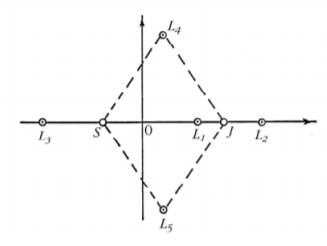
\includegraphics[scale=1.3]{f5.png}}
\caption{ Точки либрации ($О$ – центр масс тел $S$ и $J$).}
\end{figure}

Для всех точек либрации есть конечные аналитические формулы, с помощью которых можно вычислить их координаты в системе отсчета, связанной с центром масс системы. Я не буду их здесь приводить, чтобы не перегружать текст. 

В недавнее время интерес к точкам либрации возрос в связи с практически ми потребностями космических исследований. Существуют проекты запуска искусственных спутников в
окрестности точек либрации Солнечной системы. Все чаще подчеркивается важность их необычных динамических свойств с астродинамической, геофизической и эксплуатационной
точек зрения.  Были проекты создания в точках либрации баз для стоянок и техобслуживания космических станций (для проведения космических аварийно-спасательных работ, для размещения
установок по проведению технологических процессов, требующих невесомости и высокого
вакуума). Обсуждались проекты постройки в этих точках внеатмосферных астрофизических
обсерваторий и т.д. Многие из этих проектов кажутся пока фантастическими. Пока… 

Независимо от конкретных космических приложений точки либрации имеют и самостоятельный общемеханический и математический интерес. Многочисленные исследования
показали, что сами эти точки и характер движения в их окрестности тесно связаны с общим
характером движения в задаче трех тел, а это крайне важно из-за того, что общее решение задачи трех тел, как уже говорилось, не найдено. 


\paragraph{Список источников}:


$\bullet$  Алексеев В. М. Лекции по небесной механике. — Ижевск: РХД, 2001. — 156 с.

$\bullet$  Маркеев А.П. Задача трех тел и её точные решения.

$\bullet$  https://nplus1.ru/

$\bullet$  Xiaoming Li and Yipeng Jing and Shijun Liao. The 1223 new periodic orbits of planar three-body problem
with unequal mass and zero angular momentum.



\end{document}